



\newpage
\renewcommand{\thefigure}{A\arabic{figure}}
\renewcommand{\thetable}{A\arabic{table}}
\renewcommand{\theequation}{A\arabic{equation}}

\section*{Appendix} %\label{apx:demographic_model}

\section*{Demographic modeling}

Throughout we use in many ways the {\em branching process approximation} -- if an allele is locally rare, then for at least a few generations, the fates of each offspring are nearly independent.
So, if the allele is locally deleterious, the total numbers of that allele behave as a subcritical  branching process, destined for ultimate extinction.
On the other hand, if the allele is advantageous, it will either die out or become locally common, with its fate determined in the first few generations.
If the number of offspring of an individual with this allele is the random variable $X$, 
with mean $\E[X] = 1+s$ (selective advantage $s>0$), variance $\var[X]=\xi^2$, and $\P\{X=0\}>0$ (some chance of leaving no offspring),
then the probability of local nonextinction $p_*$ is approximately $p_* \approx 2s/\xi^2$ to a second order in $s$.
The precise value can be found by defining the generating function $\Phi(u) = \E[u^X]$; 
the probability of local nonextinction $p_*$ is the minimal solution to $\Phi(1-u) = 1-u$.
(This can be seen because: $1-p_*$ is the probability that an individual's family dies out;
this is equal to the probability that the families of all that individuals' children die out;
since each child's family behaves independently, if the individual has $x$ offspring, this is equal to $(1-p_*)^x$;
and $\Phi(1-p_*) = \E[(1-p_*)^X]$.)

If the selective advantage ($s$) depends on geographic location, 
a similar fact holds: index spatial location by $i \in 1, \ldots, n$,
and for $u = (u_1,u_2,\ldots,u_n)$ define the functions $\Phi_i(u) = \E[ \prod_j u_j^{X_{ij}} ]$,
where $X_{ij}$ is the (random) number of offspring that an individual at $i$ produces at location $j$.
Then $p_* = (p_{*1}, \ldots, p_{*n})$, the vector of probabilities that a new mutation at each location eventually fixes,
is the minimal solution to $\Phi(1-p_*) = 1-p_*$,
i.e.\ $\Phi_i(1-p_*) = 1-p_{*i}$.

%%%%% in rcode/maize_calcs.R
% # maize
% N <- 103359  # plants per field
% Nf <- 561    # ears to make next generation
% e <- 0.068   # prob of total seed stock replacement
% mg <- .0083  # pollen migration
% pm <- .02    # prob of partial stock addition
% m <- 0.2     # proportion of stock replaced
% eqvals <- c(1, iterroot( function (p) { 
%             p.dead <- e + (1/2)*(1-e)*(1-Nf/N)
%             return( p.dead * 1 + 
%                     (1/2)*(1-e)*exp(((1+sb)/p.dead)*( p - 1 )) + 
%                     ((1/2)*(1-e)*Nf/N)*exp(((N/Nf)*(1+sb)/(1-e))*( p - 1 )) 
%                 )
%         } ) )
% genfn <- function (f,selx,migr=.5) { 
%         (e + (1/2)*(1-e)*(1-Nf/N))* 1 + #  no offspring
%         (1/2)*(1-e)*exp(((1+selx)/(1-e))*( f + migr*diff(c(eqvals[1],f,eqvals[2]),differences=2) - 1 )) + # pollen, Poisson mean 1+s(x)
%         (1/2)*(1-e)*(Nf/N)*exp(((N/Nf)*(1+selx/(1-e)))*( f + migr*diff(c(eqvals[1],f,eqvals[2]),differences=2) - 1 )) # seed, Poisson mean (1+s(x))*N/Nf
%     }

Here we consider a linear habitat, so that the selection coefficient at location $\ell_i$ is $s_i = \min( s_b, \max( - s_d, \alpha \ell_i ) )$.
There does not seem to be a nice analytic expression for $p_*$ in this case,
but since $1-p_*$ is a fixed point of $\Phi$, the solution can be found by iteration:
$1-p_* = \lim_{n \to \infty} \Phi^n(u)$ for an appropriate starting point $u$.

\subsection*{Maize model}

The migration and reproduction dynamics we use are taken largely from \citet{vanHeerwaarden2010}.  
On a large scale,
fields of $N$ plants are replanted each year from $N_f$ ears,
either from completely new stock (with probability $p_e$),
from partially new stock (a proportion $r_m$ with probability $p_m$),
or entirely from the same field.
Plants have an average of $\mu_E$ ears per plant, and ears have an average of $N/N_f$ kernels; 
so a plant has on average $\mu_E N/N_f$ kernels, and a field has on average $\mu_E N$ ears and $\mu_E N^2/N_f$ kernels. 
%\jri{what happens if we change mean ears per plant from 3 to 1?}
%\plrnote{huh, nothing: since we assume number of ears is Poisson and the chance of replanting each ear is independent; the number of replanted ears is Poisson with a mean that is determined by the number of ears needed to replant}
We suppose that a plant with the selected allele is pollen parent to $(1+s) \mu_E N/N_f$ kernels,
and also seed parent to $(1+s)\mu_E N/N_f$ kernels, still in $\mu_E$ ears.
The number of offspring a plant has depends on how many of its offspring kernels get replanted.
Some proportion $m_g$ of the pollen-parent kernels are in other fields, and may be replanted;
but with probability $p_e$ no other kernels (i.e.~those in the same field) are replanted.
Otherwise, with probability $1-p_m$ the farmer chooses $N_f$ of the ears from this field to replant
(or, $(1-r_m) N_f$ of them, with probability $p_m$);
this results in a mean number $N_f/N$ (or, $(1-r_m)N_f/N$) of the plant's ears of seed children being chosen,
and a mean number $1+s$ of the plant's pollen children kernels being chosen.
Furthermore, the field is used to completely (or partially) replant another's field with chance $p_e/(1-p_e)$ (or $p_m$);
resulting in another $N_f/N$ (or $r_m N_f/N$) ears and $1+s$ (or $r_m (1+s)$) pollen children being replanted elsewhere.
Here we have assumed that pollen is well-mixed within a field,
and that the selected allele is locally rare.
Finally, we must divide all these offspring numbers by 2,
since we look at the offspring carrying a particular haplotype, not of the diploid plant's genome.

The above gives mean values; to get a probability model we assume that every count is Poisson.
In other words, we suppose that the number of pollen children is Poisson with random mean $\lambda_P$,
and the number of seed children is a mixture of $K$ independent Poissons with mean $(1+s)N/N_f$ each,
where $K$ is the random number of ears chosen to replant, which is itself Poisson with mean $\mu_K$.
By Poisson additivity, the numbers of local and migrant offspring are Poisson,
with means $\lambda_P = \lambda_{PL} + \lambda_{PM}$ and $\mu_K = \mu_{KL} + \mu_{KM}$ respectively.
With probability $p_e$, $\lambda_{PM} = m_g(1+s)$ and $\mu_K = \lambda_{PL} = 0$.
Otherwise, with probability $(1-p_e)(1-p_m)$, $\mu_{KL} = N_f/N$ and $\lambda_{PL} = (1+s)(1-m_g)$;
and with probability $(1-p_e)p_m$, $\mu_{KL} = (1-r_m) N_f/N$ and $\lambda_{PL} = (1-r_m)(1+s)(1-m_g)$.
The migrant means are,
with probability $(1-p_e) p_e/(1-p_e) = p_e$, $\mu_{KM} = N_f/N$ and $\lambda_{PM} = 1+s$;
while with probability $(1-p_e) p_m$, $\mu_{KM} = r_m N_f/N$ and $\lambda_{PM} = (1+s)(r_m(1-m_g) + m_g)$,
and otherwise $\mu_{KM} = 0$ and $\lambda_{PM} = m_g(1+s)$.


\begin{table}[htb!!]
  \begin{center}
  \begin{tabular}{|cll|}
    \hline
    complete seed stock replacement prob & $p_e$     & 0.068 \\
    pollen migration rate                & $m_g$      & 0.0083 \\
    number of plants per field           & $N$        & $10^5$ \\
    number of ears used to replant       & $N_f$      & 561 \\
    mean ears per plant                  & $\mu_E$    & 3 \\
    partial stock replacement prob       & $p_m$      & 0.02 \\
    mean proportion stock replaced       & $r_m$      & 0.2 \\
    pollen migration distance            & $\sigma_p$ & 0 km \\
    seed replacement distance            & $\sigma_s$ & 50 km \\
    distance between demes               & $a$        & 15 km \\
    width of altitudinal cline           & $w$        & 62km \\
    deleterious selection coefficient    & $s_d$      & varies \\
    beneficial selection coefficient     & $s_b$      & varies \\
    slope of selection gradient          & $\alpha$   & $(s_d+s_b)/w$ \\
    variance in offspring number         & $\xi^2$    & varies \\
    maize population density             & $\rho$     & $5 \times 10^3$ \\
    area of highland habitat             & $A$        & 8400 km$^2$ \\
    mean dispersal distance              & $\sigma$   & 1.8 km \\
    \hline 
  \end{tabular}
\end{center}
  \caption{Parameter estimates used in calculations, and other notation.
  \label{tab:parameters}
  }
\end{table}


\subsection*{The generating function}

The generating function of a Poisson with mean $\lambda$ is $\phi(u;\lambda)=\exp(\lambda(u-1))$,
and the generating function of a Poisson($\mu$) sum of Poisson($\lambda$) values is $\phi(\phi(u;\lambda);\mu)$.
Therefore, the generating function for the diploid process, ignoring spatial structure,
is
\begin{align}
 \Phi(u) &= \begin{aligned}[t]
   & p_e \phi(u;m_g(1+s)) \\
   & \quad {} + \left\{ (1-p_e) (1-p_m) \phi(u;(1+s)(1-m_g))\phi(\phi(u;(1+s)N/N_f);N_f/N) \right. \\
   & \quad \qquad \left. {} + (1-p_e) p_m \phi(u;(1+s)(1-r_m)(1-m_g)) \phi(\phi(u;(1+s)N/N_f);(1-r_m)N_f/N) \right\} \\
   & \quad \quad {} \times \left\{ p_e/(1-p_e) \phi(u;1+s) \phi(\phi(u;(1+s)N_f/N);N_f/N) \right. \\
   & \quad \qquad \left. {} + p_m \phi(u;(1+s)(r_m(1-p_e)(1-m_g)+m_g)) \right. \\ 
   & \quad \qquad \quad \left. {}\times \phi(\phi(u;(1+s)N/N_f);r_m N_f/N)\right. \\
   & \quad \qquad \left. {} + (1 - p_e/(1-p_e)-p_m) \phi(u;m_g(1+s)) \right\}
 \end{aligned} \label{eqn:genfn} \\
 &= \begin{aligned}[t]
   & \phi(u;m_g(1+s)) \big( \; p_e \big.\\
   & \quad {} + \left\{ (1-p_e) (1-p_m) \phi(u;(1+s)(1-m_g))\phi(\phi(u;(1+s)N/N_f);N_f/N) \right. \\
   & \quad \qquad \left. {} + (1-p_e) p_m \phi(u;(1+s)(1-r_m)(1-m_g)) \phi(\phi(u;(1+s)N/N_f);(1-r_m)N_f/N) \right\} \\
   & \quad \quad {} \times \left\{ p_e/(1-p_e) \phi(u;(1+s)(1-m_g)) \phi(\phi(u;(1+s)N_f/N);N_f/N) \right. \\
   & \quad \qquad {} + p_m \phi(u;(1+s)r_m(1-m_g)) \\
   & \quad \qquad \quad {} \times \phi(\phi(u;(1+s)N/N_f);r_m N_f/N) \\
   & \quad \qquad \left. {} + (1-p_e/(1-p_e)-p_m) \right\}  \big)
 \end{aligned}
\end{align}
To get the generating function for a haploid, replace every instance of $1+s$ by $(1+s)/2$.

As a quick check,
% \begin{align}
%   \Phi(0) &= p_e + \left\{ (1-p_e)(1-p_m)+(1-p_e)p_m \right\}
%     \times \left\{ p_e/(1-p_e) + p_m + (1-p_e/(1-p_e)-p_m) \right\}
%   &= p_e + (1-p_e)
%   &= 1 .
% \end{align}
% And, 
the mean total number of offspring of a diploid is
\begin{align}
  & \begin{aligned}
(1+s) \big(
    m_g
    + & (1-p_e)\left\{ (1-p_m) ( (1-m_g) + 1 ) + p_m ( (1-r_m)(1-m_g) + (1-r_m) ) \right\} \\
    & \qquad + \left\{ p_e ( (1-m_g) + 1 ) + p_m (1-p_e)( r_m(1-m_g) + r_m ) \right\} 
    \big) 
  \end{aligned}  \\
& \qquad = 
    (1+s) \big( m_g + 
      (1-p_e)(2-m_g)(1 - p_m r_m)
      + ( p_e (2-m_g) + p_m r_m (1-p_e)(2-m_g) )
    \big) \\
& \qquad = (1+s) \big( 
    m_g + (2-m_g) ( (1-p_e) (1 - p_m r_m) + p_e + p_m r_m(1-p_e) )
  \big) \\
& \qquad = (1+s) \big( 
    m_g + (2-m_g)
  \big) \\
& \qquad = 2(1+s) .
\end{align}

We show numerically later that the probability of establishment is very close to $2s$ over the variance in reproductive number (as expected).
It is possible to write down an expression for the variance, 
but the exact expression does not aid the intuition.

\subsection*{Migration and spatial structure}

To incorporate spatial structure, suppose that the locations $\ell_k$ are arranged in a regular grid, so that $\ell_k = a k$. 
Recall that $s_k$ is the selection coefficient at location $k$.
If the total number of offspring produced by an individual at $\ell_i$ is Poisson($\lambda_i$), with each offspring independently migrating to location $j$
with probability $m_{ij}$,
then the number of offspring at $j$ is Poisson($m_{ij}\lambda_i$),
and so the generating function is
\begin{align}
  \phi(u;\lambda,m) &= \prod_j \exp( \lambda_i m_{ij} ( u_j - 1 ) ) \\
  &= \exp\left\{ \lambda_i \left(\left(\sum_j m_{ij} u_j\right) - 1\right) \right\} .
\end{align}
We can then substitute this expression into equation \eqref{eqn:genfn},
with appropriate migration kernels for pollen and seed dispersal.

For migration, we need migration rates and migration distances for both wind-blown pollen
and for farmer seed exchange.
The rates are parameterized as above;
we need the typical dispersal distances, however.
One option is to say that the typical distance between villages is $d_v$,
and that villages are discrete demes,
so that pollen stays within the deme (pollen migration distance 0)
and seed is exchanged with others from nearby villages;
on average $\sigma_s$ distance away in a random direction.
The number of villages away the seed comes from could be geometric 
(including the possibility of coming from the same village).

\subsection*{Dispersal distance}

The dispersal distance
-- the mean distance between parent and offspring --
is equal to the chance of inter-village movement
multiplied by the mean distance moved.
This is
% pe <- .068; pm <- .02; rm <- .2; sigma.s <- 50
% (pe + (1-pe)*pm*rm) * sigma.s
\begin{align}
  \sigma = (p_e + (1-p_e) p_m r_m ) \sigma_s = 3.5864 \text{km}
\end{align}
at the parameter values above.

Iterating the generating function above finds the probability of establishment as a function of distance along the cline.
This is shown in figure \ref{sfig:prob_estab}.
Note that the approximation $2s$ divided by the variance in offspring number is quite close.

\begin{figure}[ht!!]
  \begin{center}
    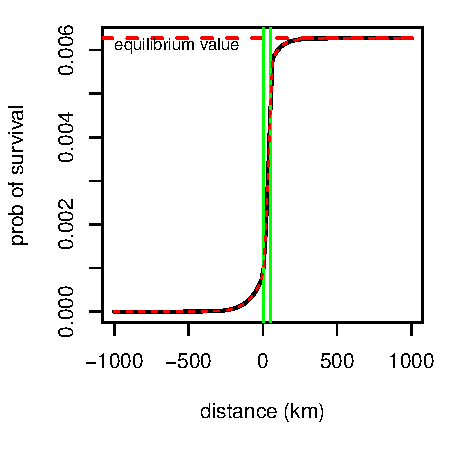
\includegraphics{prob-estab-62}
    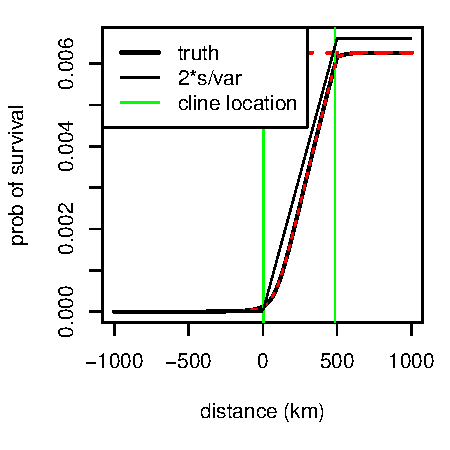
\includegraphics{prob-estab-500}
  \end{center}
  \caption{
  Probability of establishment, as a function of distance along and around an altitudinal cline, whose boundaries are marked by the green lines.
  {\bf (A)} The parameters above; with cline width 62km; {\bf (B)} the same, except with cline width 500km.
  \label{sfig:prob_estab}
  }
\end{figure}


In the main text, we used a rough upper bound on the rate of migration
that ignored correlations in migrants.
As we show in \citet{ralph2014convergent}, 
the rate of adaptation by diffusive migration is more precisely
\begin{align*}
  \migrate = \frac{1}{2} \rho s_m \min(s_m,2s_b/\xi^2) \exp\left(- \frac{\sqrt{2 s_m}R}{\sigma} \right) .
\end{align*}

%\jri{do we need to explain? not sure.}
%\plrnote{we could just cut the remining discussion.}
%But for now, let's interpret.

First note that for $10^{-1} \le s_m \le 10^{-4}$, the value $1/\sqrt{2s_m}$ is between 2 and 70 --
so the exponential decay of the chance of migration falls off on a scale of between 2 and 70 times the dispersal distance.
Above we have estimated the dispersal distance to be $\sigma \approx 3.5$ km,
and far below the mean distance $\sigma_s$ to the field that a farmer replants seed from, when this happens,
which we have as $\sigma_s = 50$ km.
Taking $\sigma=3.5$ km, we have that $7 \le \sigma/\sqrt{2s_m} \le 250$ km.
A very conservative upper bound might be $\sigma \le \sigma_s/10$ (if farmers replaced 10\% of their seed with long-distance seed every year).
At this upper bound, we would have $10 \le \sigma/\sqrt{2s_m} \le 350$ km,
which is not very different.
This makes the exponential term small since $R$ is on the order of thousands of kilometers.

% rho <- 5000; xisq <- 30; sigma <- 3.5
% params <- expand.grid( R=1000*(1:4), sm=10^(-(1:4)) )
% params$char.length <- with(params, sigma/sqrt(2*sm) )
% params$migrate <- with( params, ( ( rho * sb * pmin(sm,2*sb/xisq) / 2 )* exp(- sqrt(2*sm)*R/sigma ) ) )
% params$Tmig <- with( params, 1/migrate )
% print(params)

Taking $\sigma=3.5$ km, we then compute that 
if $s_m = 10^{-4}$ (very weak selection in the lowlands), then for $R=1,000$ km, the migration rate is $\migrate \le 10^{-5}$,
i.e.\ it would take on the order of 100,000 generations (years) to get a successful migrant only 1,000 km away,
under this model of undirected, diffusive dispersal.
For larger $s_m$, the migration rate is much smaller.


%%%%%%%%%%%%%
\subsection*{Migration rate of deleterious alleles}

\rev{
In the main text we computed $\migrate$, the rate at which new adaptive alleles appeared by mutation.
A corresponding expression for the chance that an allele moves from one highland population to another is harder to intuit.
This problem is studied in more depth in \cite{ralph2014convergent},
under the assumption that the alleles are deleterious between the highlands.
Since such deleterious alleles are much less likely to transit than neutral ones,
the analysis in the main text implies that gene flow is unlikely to have shared these alleles between highland regions.
However, because spatially continuous models assuming selective effects are better understood than neutral ones,
and we do expect a tradeoff between highland- and lowland-adaptation,
it is useful to understand what happens in this case as well.
}

If an allele is beneficial at high elevation and fixed in the Mesoamerican highlands but is deleterious at low elevations, 
then at equilibrium it will be present at low frequency at migration-selection balance in nearby lowland populations \citep{haldane1948theory,slatkin1973geneflow}.
This equilibrium frequency decays exponentially with distance, so that the highland allele is present at distance $R$ from the highlands at frequency $C \exp(- R \sqrt{2s_m} / \sigma)$, where $s_m$ is the deleterious selection coefficient for the allele in low elevation, $\sigma$ is the mean dispersal distance, and $C$ is a constant depending on geography ($C\approx 1/2$ is close).
Multiplying this frequency by a population size gets the predicted number (average density across a large number of generations) of individuals carrying the allele.
Therefore, in a lowland population of size $N$ at distance $R$ from the highlands, $(N/2)  \exp(- R \sqrt{2s_m} / \sigma)$ 
is equal to the probability that there are any highland alleles present, multiplied by the expected number of these given that some are present.
Since we assume the allele is deleterious in the lowlands, if $R$ is large there are likely none present;
but if there are, the expected number is of order $1/s_m$ \citep{geiger1999elementary,ralph2014convergent}.
This therefore puts an upper bound on the rate of migration of
\begin{align} \label{eqn:migrate}
  \migrate \le (s_m N/2)  \exp(- R \sqrt{2s_m} / \sigma),
\end{align}
and we we would need to wait $\Tmig = 1/\migrate$ generations for a rare such excursion to occur.
This calculation omits the probability that such an allele fixes ($\approx 2s_b/\xi^2$)
(discussed above)
and the time to reach migration-selection balance
(discussed in the main text);
both of these omissions mean we underestimate $\Tmig$.


\paragraph{Results for gene flow of deleterious alleles:}
From our demographic model we have estimated a mean dispersal distance of $\sigma \approx 3.5$ kilometers per generation.
With selection against the highland allele in low elevations $10^{-1} \ge s_m \ge 10^{-4}$, 
the distance $\sigma/\sqrt{2s_m}$ over which the frequency of a highland-adaptive, lowland-deleterious allele decays into the lowlands is still short: 
between 7 and 250 kilometers.
Since the Mesoamerican and Andean highlands are around 4,000 km apart, 
the time needed for a rare allele with weak selective cost $s_m=10^{-4}$ in the lowlands 
to transit between the two highland regions is $\Tmig \approx 8 \times 10^{4}$ generations. 
While the exponential dependence on distance in equation \eqref{eqn:migrate} means that shorter distances could be transited more quickly, the waiting time $\Tmig$ is also strongly dependent on the magnitude of the deleterious selection coefficient: with $s_m=10^{-4}$, $\Tmig \approx 25$ generations over a distance of 2,000 km, but increases to $\approx 10^{8}$ generations with a still weak selective cost of $s_m=10^{-3}$.
%, however: with the still weak selective cost of $s_m=10^{-3}$, for example, $\Tmig$ is $10^8$ generations over 2,000km,
%-- if the distance between highland patches is 2,000 km (or if $\sigma$ is twice as large) then $\Tmig \approx 25$ generations, indicating that all alleles beneficial in both highlands but with such weak selection cost in the lowlands should be shared if they arose long enough ago for migration-selection balance to have been reached.
%and much larger for longer distances.

%\plrnote{The above has changed because I found an factor of 2 missed out in $\sigma$, 
%and the R code has an factor of $2s_b/\xi^2$ that wasn't present in \eqref{eqn:migrate}.
%This is an overestimate of the rate that is more correctly given in the supplement;
%I didn't worry about this before, when migration was unlikely for all parameter values.
%However, now $\Tmig$ is smallish for $R=1,000$ and $s_m=10^{-3}$ with the approximation \eqref{eqn:migrate},
%but not with the better expression of the appendix.
%This makes me want to put in the better expression, which I can't quickly motivate,
%except that the next bit makes it not matter, I think.}




\newpage


\setcounter{table}{0} %% DON'T REMOVE
\setcounter{figure}{0}%% DON'T REMOVE

%\clearpage

% space of double hline in Table
\doublerulesep = 0.4pt

%\section*{SUPPLEMENTAL METHODS}
\renewcommand{\thefigure}{S\arabic{figure}}
\renewcommand{\thetable}{S\arabic{table}}


%%%%%%%%%%%%%%%%%%%%%%%%%%%%%%%
%Table S1 %
\renewcommand{\arraystretch}{1.2}

\begin{table}[h]
    \begin{center}
    \caption[]{List of maize landraces used in this study\hspace*{9.1cm}}  
{\fontsize{7}{10}\selectfont
%{\small
    \begin{tabular}{llllllllll}
        \hline\hline
       & & & \\[-4mm] 
	 ID$^a$	&	USDA ID	&	Population	&	Landrace	&	Locality	&	Latitude	&	Longitude	&	Elevation	&	Origin	\\[0.0cm]
	\hline 
	& & & \\[-4mm] 
{\bf RIMMA0409}	&	PI 478968	&	Mesoamerican 	&	Tepecintle	&	Chiapas, Mexico	&	15.4 	&	-92.9 	&	107	&	USDA	\\
RIMMA0410	&	PI 478970	&	Lowland	&	Vandeno	&	Chiapas, Mexico	&	15.4 	&	-92.9 	&	107	&	USDA	\\
{\bf RIMMA0433}	&	PI 490825	&		&	Nal Tel ATB	&	Chiquimula, Guatemala	&	14.7 	&	-89.5 	&	457	&	USDA	\\
{\bf RIMMA0441}	&	PI 515538	&		&	Coscomatepec	&	Veracruz, Mexico	&	19.2 	&	-97.0 	&	1320	&	USDA	\\
{\bf RIMMA0615}	&	PI 628480	&		&	Tuxpeno	&	Puebla, Mexico	&	20.1 	&	-97.2 	&	152	&	USDA	\\
{\bf RIMMA0619}	&	PI 645772	&		&	Pepitilla	&	Guerrero, Mexico	&	18.4 	&	-99.5 	&	747	&	USDA	\\
{\bf RIMMA0628}	&	PI 646017	&		&	Tuxpeno Norteno	&	Tamaulipas, Mexico	&	23.3 	&	-99.0 	&	300	&	USDA	\\
{\bf RIMMA0696}	&	Ames 28568	&		&	Tuxpeno	&	El Progreso, Guatemala	&	16.5 	&	-90.2 	&	30	&	Goodman	\\
{\bf RIMMA0700}	&	NSL 291626	&		&	Olotillo	&	Chiapas, Mexico	&	16.8 	&	-93.2 	&	579	&	Goodman	\\
{\bf RIMMA0701}	&	PI 484808	&		&	Olotillo	&	Chiapas, Mexico	&	16.6 	&	-92.7 	&	686	&	Goodman	\\
{\bf RIMMA0702}	&	Ames 28534	&		&	Negro de Tierra Caliente	&	Sacatepequez, Guatemala	&	14.5 	&	-90.8 	&	1052	&	Goodman	\\
{\bf RIMMA0703}	&	NSL 283390	&		&	Nal Tel	&	Yucatan, Mexico	&	20.8 	&	-88.5 	&	30	&	Goodman	\\
{\bf RIMMA0709}	&	Ames 28452	&		&	Tehua	&	Chiapas, Mexico	&	16.5 	&	-92.5 	&	747	&	Goodman	\\
{\bf RIMMA0710}	&	PI 478988	&		&	Tepecintle	&	Chiapas, Mexico	&	15.3 	&	-92.6 	&	91	&	Goodman	\\
{\bf RIMMA0712}	&	NSL 291696 CYMT	&		&	Oloton	&	Baja Verapaz, Guatemala	&	15.3 	&	-90.3 	&	1220	&	Goodman	\\
{\bf RIMMA0716}	&	Ames 28459	&		&	Zapalote Grande	&	Chiapas, Mexico	&	15.3 	&	-92.7 	&	91	&	Goodman	\\
{\bf RIMMA0720}	&	PI 489372	&		&	Negro de Tierra Caliente	&	Guatemala	&	15.5 	&	-88.9 	&	39	&	Goodman	\\
{\bf RIMMA0721}	&	Ames 28485	&		&	Nal Tel ATB	&	Chiquimula, Guatemala	&	14.6 	&	-90.1 	&	915	&	Goodman	\\
{\bf RIMMA0722}	&	Ames 28564	&		&	Dzit Bacal	&	Jutiapa, Guatemala	&	14.3 	&	-89.7 	&	737	&	Goodman	\\
{\bf RIMMA0727}	&	Ames 28555	&		&	Comiteco	&	Guatemala	&	14.4 	&	-90.5 	&	1151	&	Goodman	\\
{\bf RIMMA0729}	&	PI 504090	&		&	Tepecintle	&	Guatemala	&	15.4 	&	-89.7 	&	122	&	Goodman	\\
{\bf RIMMA0730}	&	Ames 28517	&		&	Quicheno Late	&	Sacatepequez, Guatemala	&	14.5 	&	-90.8 	&	1067	&	Goodman	\\
{\bf RIMMA0731}	&	PI 484137	&		&	Bolita	&	Oaxaca, Mexico	&	16.8 	&	-96.7 	&	1520	&	Goodman	\\
{\bf RIMMA0733}	&	PI 479054	&		&	Zapalote Chico	&	Oaxaca, Mexico	&	16.6 	&	-94.6 	&	107	&	Goodman	\\
	\hline 
	& & & \\[-4mm] 
{\bf RIMMA0416}	&	PI 484428	&	Mesoamerican	&	Cristalino de Chihuahua	&	Chihuahua, Mexico	&	29.4 	&	-107.8 	&	2140	&	NA	\\
{\bf RIMMA0417}	&	PI 484431	&	Highland	&	Azul	&	Chihuahua, Mexico	&	28.6 	&	-107.5 	&	2040	&	USDA	\\
{\bf RIMMA0418}	&	PI 484476	&		&	Gordo	&	Chihuahua, Mexico	&	28.6 	&	-107.5 	&	2040	&	USDA	\\
{\bf RIMMA0421}	&	PI 484595	&		&	Conico	&	Puebla, Mexico	&	19.9 	&	-98.0 	&	2250	&	USDA	\\
{\bf RIMMA0422}	&	PI 485071	&		&	Elotes Conicos	&	Puebla, Mexico	&	19.1 	&	-98.3 	&	2200	&	USDA	\\
{\bf RIMMA0423}	&	PI 485116	&		&	Cristalino de Chihuahua	&	Chihuahua, Mexico	&	29.2 	&	-108.1 	&	2095	&	NA	\\
{\bf RIMMA0424}	&	PI 485120	&		&	Apachito	&	Chihuahua, Mexico	&	28.0 	&	-107.6 	&	2400	&	USDA	\\
{\bf RIMMA0425}	&	PI 485128	&		&	Palomero Tipo Chihuahua	&	Chihuahua, Mexico	&	26.8 	&	-107.1 	&	2130	&	USDA	\\
{\bf RIMMA0614}	&	PI 628445	&		&	Mountain Yellow	&	Jalisco, Mexico	&	20.0 	&	-103.8 	&	2060	&	USDA	\\
{\bf RIMMA0616}	&	PI 629202	&		&	Zamorano Amarillo	&	Jalisco, Mexico	&	20.8 	&	-102.8 	&	1800	&	USDA	\\
{\bf RIMMA0620}	&	PI 645786	&		&	Celaya	&	Guanajuato, Mexico	&	20.2 	&	-100.9 	&	1799	&	USDA	\\
{\bf RIMMA0621}	&	PI 645804	&		&	Zamorano Amarillo	&	Guanajuato, Mexico	&	21.1 	&	-101.7 	&	1870	&	USDA	\\
{\bf RIMMA0623}	&	PI 645841	&		&	Palomero de Jalisco	&	Jalisco, Mexico	&	20.0 	&	-103.7 	&	2520	&	USDA	\\
{\bf RIMMA0625}	&	PI 645984	&		&	Cacahuacintle	&	Puebla, Mexico	&	19.0 	&	-97.4 	&	2600	&	USDA	\\
RIMMA0626	&	PI 645993	&		&	Arrocillo Amarillo	&	Puebla, Mexico	&	19.9 	&	-97.6 	&	2260	&	USDA	\\
{\bf RIMMA0630}	&	PI 646069	&		&	Arrocillo Amarillo	&	Veracruz, Mexico	&	19.8 	&	-97.3 	&	2220	&	USDA	\\
{\bf RIMMA0670}	&	Ames 28508	&		&	San Marceno	&	San Marcos, Guatemala	&	15.0 	&	-91.8 	&	2378	&	Goodman	\\
{\bf RIMMA0671}	&	Ames 28538	&		&	Salpor Tardio	&	Solola, Guatemala	&	14.8 	&	-91.3 	&	2477	&	Goodman	\\
{\bf RIMMA0672}	&	PI 483613	&		&	Chalqueno	&	Mexico, Mexico	&	19.7 	&	-99.1 	&	2256	&	Goodman	\\
{\bf RIMMA0674}	&	PI 483617	&		&	Toluca	&	Mexico, Mexico	&	19.3 	&	-99.7 	&	2652	&	Goodman	\\
{\bf RIMMA0677}	&	Ames 28476 	&		&	Conico Norteno	&	Zacatecas, Mexico	&	21.4 	&	-102.9 	&	1951	&	Goodman	\\
{\bf RIMMA0680}	&	Ames 28448	&		&	Tabloncillo	&	Jalisco, Mexico	&	20.4 	&	-102.2 	&	1890	&	Goodman	\\
{\bf RIMMA0682}	&	PI 484571	&		&	Tablilla de Ocho	&	Jalisco, Mexico	&	22.1 	&	-103.2 	&	1700	&	Goodman	\\
{\bf RIMMA0687}	&	Ames 28473	&		&	Conico Norteno	&	Queretaro, Mexico	&	20.4 	&	-100.0 	&	1921	&	Goodman	\\[-0.1mm]	
	                         %&                       &                                 & \emph{BoS-68}  & AB298905       &  AB054737\\[-0.1mm]	
	\hline\hline
\multicolumn{9}{l}{$^a$ GBS data are available for the accessions in bold font.}\\
    \end{tabular}}

\end{center} 

\end{table}

\clearpage
%%%%%%%%%%%%%%%%%%%%%%%%%%%%%%%%%%%%%%%%%%%

\setcounter{table}{0}
%%%%%%%%%%%%%%%%%%%%%%%%%%%%%%%
%Table S1 %
\renewcommand{\arraystretch}{1.2}

\begin{table}[h]
    \begin{center}
    \caption[]{(continued)\hspace*{13.5cm}}  
{\fontsize{7}{10}\selectfont
%{\small
    \begin{tabular}{llllllllll}
        \hline\hline
       & & & \\[-4mm] 
	 ID	&	USDA ID	&	Population	&	Landrace	&	Locality	&	Latitude	&	Longitude	&	Elevation (m)	&	Origin	\\[0.0cm]
	\hline 
	& & & \\[-4mm] 
{\bf RIMMA0388}	&	PI 443820	&	S. American	&	Amagaceno	&	Antioquia, Colombia	&	6.9 	&	-75.3 	&	1500	&	USDA	\\
{\bf RIMMA0389}	&	PI 444005	&	Lowland	&	Costeno	&	Atlantico, Colombia	&	10.4 	&	-74.9 	&	7	&	USDA	\\
{\bf RIMMA0390}	&	PI 444254	&		&	Comun	&	Caldas, Colombia	&	4.5 	&	-75.6 	&	353	&	USDA	\\
RIMMA0391	&	PI 444296	&		&	Andaqui	&	Caqueta, Colombia	&	1.4 	&	-75.8 	&	700	&	USDA	\\
{\bf RIMMA0392}	&	PI 444309	&		&	Andaqui	&	Caqueta, Colombia	&	1.8 	&	-75.6 	&	555	&	USDA	\\
{\bf RIMMA0393}	&	PI 444473	&		&	Costeno	&	Cordoba, Colombia	&	8.3 	&	-75.2 	&	100	&	USDA	\\
{\bf RIMMA0394}	&	PI 444621	&		&	Pira	&	Cundinamarca, Colombia	&	4.8 	&	-74.7 	&	1000	&	USDA	\\
{\bf RIMMA0395}	&	PI 444731	&		&	Negrito	&	Choco, Colombia	&	8.5 	&	-77.3 	&	30	&	USDA	\\
{\bf RIMMA0396}	&	PI 444834	&		&	Caqueteno	&	Huila, Colombia	&	2.6 	&	-75.3 	&	1100	&	USDA	\\
{\bf RIMMA0397}	&	PI 444897	&		&	Negrito	&	Magdalena, Colombia	&	11.6 	&	-72.9 	&	50	&	USDA	\\
{\bf RIMMA0398}	&	PI 444923	&		&	Puya	&	Magdalena, Colombia	&	9.4 	&	-75.7 	&	27	&	USDA	\\
{\bf RIMMA0399}	&	PI 444954	&		&	Cariaco	&	Magdalena, Colombia	&	10.2 	&	-74.1 	&	250	&	USDA	\\
{\bf RIMMA0403}	&	PI 445163	&		&	Pira Naranja	&	Narino, Colombia	&	1.3 	&	-77.5 	&	1000	&	USDA	\\
{\bf RIMMA0404}	&	PI 445322	&		&	Puya Grande	&	Norte de Santander, Colombia	&	7.3 	&	-72.5 	&	1500	&	USDA	\\
RIMMA0405	&	PI 445355	&		&	Puya	&	Norte de Santander, Colombia	&	8.4 	&	-73.3 	&	1100	&	USDA	\\
{\bf RIMMA0406}	&	PI 445514	&		&	Yucatan	&	Tolima, Colombia	&	5.0 	&	-74.9 	&	450	&	USDA	\\
RIMMA0407	&	PI 445528	&		&	Pira	&	Tolima, Colombia	&	4.2 	&	-74.9 	&	450	&	USDA	\\
{\bf RIMMA0428}	&	PI 485354	&		&	Aleman	&	Huanuco, Peru	&	-9.3 	&	-76.0 	&	700	&	NA	\\
{\bf RIMMA0462}	&	PI 445073	&		&	Amagaceno	&	Narino, Colombia	&	1.6 	&	-77.2 	&	1700	&	USDA	\\
{\bf RIMMA0690}	&	PI 444946	&		&	Puya	&	Magdalena, Colombia	&	8.3 	&	-73.6 	&	250	&	Goodman	\\
{\bf RIMMA0691}	&	PI 445391	&		&	Cacao	&	Santander, Colombia	&	6.6 	&	-73.1 	&	1098	&	NA	\\
{\bf RIMMA0707}	&	PI 487930	&		&	Tuxpeno	&	Ecuador	&	-1.1 	&	-80.5 	&	30	&	Goodman	\\
{\bf RIMMA0708}	&	PI 488376	&		&	Yunquillano F Andaqui	&	Ecuador	&	-3.5 	&	-78.6 	&	1098	&	Goodman	\\
	\hline 
	& & & \\[-4mm] 
{\bf RIMMA0426}	&	PI 485151	&	S. American	&	Rabo de Zorro	&	Ancash, Peru	&	-9.1 	&	-77.8 	&	2500	&	NA	\\
{\bf RIMMA0430}	&	PI 485362	&	Highland	&	Sarco	&	Ancash, Peru	&	-9.2 	&	-77.7 	&	2585	&	NA	\\
{\bf RIMMA0431}	&	PI 485363	&	 	&	Perlilla	&	Huanuco, Peru	&	-8.7 	&	-77.1 	&	2900	&	NA	\\
{\bf RIMMA0436}	&	PI 514723	&		&	Morocho Cajabambino	&	Amazonas, Peru	&	-6.2 	&	-77.9 	&	2200	&	NA	\\
{\bf RIMMA0437}	&	PI 514752	&		&	Ancashino	&	Ancash, Peru	&	-9.3 	&	-77.6 	&	2688	&	NA	\\
{\bf RIMMA0438}	&	PI 514809	&		&	Maranon	&	Ancash, Peru	&	-8.7 	&	-77.4 	&	2820	&	NA	\\
RIMMA0439	&	PI 514969	&		&	Maranon	&	La Libertad, Peru	&	-8.5 	&	-77.2 	&	2900	&	NA	\\
{\bf RIMMA0464}	&	PI 571438	&		&	Chullpi	&	Huancavelica, Peru	&	-12.3 	&	-74.7 	&	1800	&	USDA	\\
{\bf RIMMA0465}	&	PI 571457	&		&	Huarmaca	&	Piura, Peru	&	-5.6 	&	-79.5 	&	2300	&	USDA	\\
{\bf RIMMA0466}	&	PI 571577	&		&	Confite Puneno	&	Apurimac, Peru	&	-14.3 	&	-72.9 	&	3600	&	USDA	\\
{\bf RIMMA0467}	&	PI 571871	&		&	Paro	&	Apurimac, Peru	&	-13.6 	&	-72.9 	&	2800	&	USDA	\\
{\bf RIMMA0468}	&	PI 571960	&		&	Sarco	&	Ancash, Peru	&	-9.4 	&	-77.2 	&	3150	&	USDA	\\
{\bf RIMMA0473}	&	PI 445114	&		&	Sabanero	&	Narino, Colombia	&	1.1 	&	-77.6 	&	3104	&	USDA	\\
{\bf RIMMA0656}	&	Ames 28799	&		&	Culli	&	Jujuy, Argentina	&	-23.2 	&	-65.4 	&	2287	&	Goodman	\\
{\bf RIMMA0657}	&	NSL 286594	&		&	Chake Sara	&	Bolivia	&	-17.5 	&	-65.7 	&	2201	&	Goodman	\\
{\bf RIMMA0658}	&	NSL 286812	&		&	Uchuquilla	&	Bolivia	&	-21.8 	&	-64.1 	&	1948	&	Goodman	\\
{\bf RIMMA0661}	&	PI 488066	&		&	Chillo	&	Ecuador	&	-2.9 	&	-78.7 	&	2195	&	Goodman	\\
{\bf RIMMA0662}	&	NSL 287008	&		&	Cuzco	&	Ecuador	&	0.0 	&	-78.0 	&	2195	&	Goodman	\\
{\bf RIMMA0663}	&	PI 488102	&		&	Mishca	&	Ecuador	&	0.4 	&	-78.2 	&	2067	&	Goodman	\\
{\bf RIMMA0664}	&	PI 488113	&		&	Blanco Blandito	&	Ecuador	&	0.4 	&	-78.4 	&	2122	&	Goodman	\\
{\bf RIMMA0665}	&	PI 489324	&		&	Racimo de Uva	&	Ecuador	&	-0.9 	&	-78.9 	&	2931	&	Goodman	\\
{\bf RIMMA0667}	&	Ames 28737	&		&	Patillo	&	Chuquisaca, Bolivia	&	-21.8 	&	-64.1 	&	2201	&	NA	\\
RIMMA0668	&	Ames 28668	&		&	Granada	&	Puno, Peru	&	-14.9 	&	-70.6 	&	3925	&	Goodman	\\[-0.1mm] 
	                         %&                       &                                 & \emph{BoS-68}  & AB298905       &  AB054737\\[-0.1mm]	
	\hline\hline
	\multicolumn{9}{l}{$^a$ GBS data are available for the accessions in bold font.}\\
    \end{tabular}}
    \label{srkid}

\end{center} 

\end{table}

\clearpage
%%%%%%%%%%%%%%%%%%%%%%%%%%%%%%%%%%%%%%%%%%%




%%%%%%%%%%%%%%%%%%%%%%%%%%%%%%%%%%%%%%%%%%%%%%%%%%%%%%%%%%%%
%\renewcommand{\arraystretch}{1.1}
%\begin{table}[h]
%
%\begin{center}
% \caption[]{Inference of demographic parameters \st{(Remove this table later.)}\hspace*{0.3cm}}
%  \textbf{}\\[-2mm]
%{\fontsize{8}{11}\sf
%    \begin{tabular}{ccccccccl} \hline\hline
%       & & \\[-3mm]
%     Mesoamerica  & \multicolumn{2}{c}{Model IA}  \\[0.1cm]
%    \hline
%    & & \\[-3mm]
%   & Likelihood & $-$3052.34  \\
%  &$N_B$ & 148,500 \\
%  &$N_C$ & 148,500 \\   
%  &$N_1$ & 62,370 \\ 
%  &$N_2$ & 86,130 \\ 
%  &$N_{2P}$   & 86,130    \\ 
%      \hline
%    & & \\[-3mm]
%    S. America  & \multicolumn{2}{c}{Model IA}  \\[0.1cm]
%        \hline
%    & & \\[-3mm]
%     & Likelihood &  $-$2717.64  \\
%       &$N_B$ & 76,500 \\     	
%       &$N_C$ & 76,500 \\
%      &$N_1$ & 74,205           \\ 
%      &$N_2$ & 2,295       \\      
%      &$N_{2P}$   & 346,545   \\[1mm]
%    \hline\hline
%\multicolumn{3}{l}{The description of $\alpha, \beta$ and $\gamma$ is in Figure~3.}\\
%\multicolumn{3}{l}{$\sigma$ is a relative size of $N_B$ to $N_C$ ($N_B=\sigma N_C$).}\\
%    \end{tabular}
%    \label{supp:param}  % caption is needed to make this work
%}
%\end{center}
%\end{table}
%\renewcommand{\arraystretch}{1}
%%%%%%%%%%%%%%%%%%%%%%%%%%%%%%%%%%%%%%%%%%%%%%%%%%%%%%%%%%%%


%%%%%%%%%%%%%%%%%%%%%%%%%%%%%%%%%%%%%%%%%%%%%%%%%%%%%%%%%%%%
\renewcommand{\arraystretch}{1.1}
\begin{table}[h]

\begin{center}
 \caption[]{Summary of PHS test\hspace*{9.1cm}}
  \textbf{}\\[-2mm]
{\fontsize{8}{11}\sf
    \begin{tabular}{lllllcccccl} \hline\hline
       & & \\[-3mm]
     Population  & Pattern of adaptation & No. of SNPs & No. of SNPs supported by PHS test & \st{Significance $^a$} \\[0.1cm]
    \hline
    & & \\[-3mm]
   Mesoamerica & Highland adaptation & 264 & 172 (65.2\%) &  $P<10^{-3}$ \\
               & Lowland adaptation & 101 & 66 (65.3\%) & $P<0.05$ \\
   S. America & Highland adaptation & 164 & 230 (71.3\%) &  $P<10^{-5}$  \\
                     & Lowland adaptation & 70 & 50 (71.4\%)  & $P<0.05$ \\[0.1cm]
    \hline\hline
    \multicolumn{5}{l}{\rev{$^a$ Probability of the observed percent of SNPs showing a lower empirical quantile. Under neutrality, 50\% of SNPs should have lower PHS values in the focal population; higher values indicate evidence of selection.  See the main text for details. }}\\
    \end{tabular}
    \label{supp:phs}  % caption is needed to make this work
}
\end{center}
\end{table}
\renewcommand{\arraystretch}{1}
%%%%%%%%%%%%%%%%%%%%%%%%%%%%%%%%%%%%%%%%%%%%%%%%%%%%%%%%%%%%

%%%%%%%%%%%%%%%%%%%%%%%%%%%%%%%%%%%%%%%%%%%%%%%%%%%%%%%%%%%%=
\begin{table}[h]	
	\caption[]{\st{List of metabolic pathways showing evidence of convergent adaptation}\hspace*{0.3cm}} 
			\centering
			\textbf{}\\[-2mm]
			{\fontsize{7}{11}\sf
		    \begin{tabular}{l} \hline\hline\\[-3mm]
		    Colanic acid building blocks biosynthesis\\
		    Purine nucleotides \textit{de novo} biosynthesis II\\	    
		    Adenosine nucleotides \textit{de novo} biosynthesis\\
NAD/NADH phosphorylation and dephosphorylation\\
tRNA charging pathway\\
Superpathway of phenylalanine biosynthesis\\
Superpathway of tryptophan biosynthesis\\
Aspartate biosynthesis\\
Tryptophan biosynthesis\\
Glutamine biosynthesis III\\
Isoleucine biosynthesis I\\
Threonine biosynthesis\\
Galactose degradation III\\
UDP-glucose biosynthesis (from glucose 6-phosphate)\\
Triacylglycerol biosynthesis\\
Phospholipid biosynthesis II\\
Phosphatidylglycerol biosynthesis I (plastidic)\\
Phosphatidylglycerol biosynthesis II (non-plastidic)\\
CDP-diacylglycerol biosynthesis II\\
CDP-diacylglycerol biosynthesis I\\
Ethylene biosynthesis from methionine\\
Stachyose degradation\\
Homogalacturonan degradation\\
Betanidin degradation\\
Aspartate degradation II\\
Phosphate utilization in cell wall regeneration\\
Phosphate acquisition\\
Superpathway of cytosolic glycolysis (plants), pyruvate dehydrogenase and TCA cycle\\
C4 photosynthetic carbon assimilation cycle\\
Glycolysis IV (plant cytosol)\\
Glycolysis I\\
Glycolysis III\\
		      \hline\hline
		    \end{tabular}
		    \label{supp:metabo}  % caption is needed to make this work
		}
\end{table}
%%%%%%%%%%%%%%%%%%%%%%%%%%%%%%%%%%%%%%%%%%%%%%%%%%%%%%%%%%%%

%%%%%%%%%%%%%%%%%%%%%%%%%%%%%%%%%%%%%%%%%%%%%%%%%%%%%%%%%%%%
\renewcommand{\arraystretch}{1.1}
\begin{table}[h]

\begin{center}
 \caption[]{$F_{CT}$ between \emph{parviglumis} and \emph{mexicana}\hspace*{0.3cm}}
  \textbf{}\\[-2mm]
{\fontsize{7}{11}\sf
    \begin{tabular}{lcccccccl} 
    \hline\hline
       
Mesoamerica     & \multicolumn{3}{c}{No. of SNPs}  \\
                                  & Significant & NS          & Proportion  \\
Significant $F_{CT}$ & 25              &   337       & 0.077\\ 
NS                             & 299            &  18,493   & 0.018\\
      \hline
    & & \\[-3mm]
S. America     & \multicolumn{3}{c}{No. of SNPs} \\
                                     & Significant & NS           & Proportion  \\
Significant $F_{CT}$    & 10              &   327        & 0.070\\ 
NS                                & 133            &  17,518    & 0.018\\[1mm]
    \hline\hline
  %\multicolumn{4}{l}{$^{a}$ \textcolor{red}{Maybe we should use the number of genetic unit.}}\\
  % \multicolumn{4}{l}{$^{a}$ \textcolor{red}{Sum of the number of SNPs != 91,779 because I excluded SNPs exhibiting}}\\[-0.5mm]
  % \multicolumn{4}{l}{ \textcolor{red}{     monomorphic in Mexico or in South America.}}\\
    \end{tabular}
    \label{tanja}  % caption is needed to make this work
}
\end{center}
\end{table}
\renewcommand{\arraystretch}{1}
%%%%%%%%%%%%%%%%%%%%%%%%%%%%%%%%%%%%%%%%%%%%%%%%%%%%%%%%%%%%


%%%%%%%%%%%%%%%%%%%%%%%%%%%%%%%%%%%%%%%%%%%%%%%%%%%%%%%%%%%%=
\begin{table}[h]	
	\caption[]{$F_{ST}$ outlier SNPs and \emph{mexicana} introgression\hspace*{0.3cm}} 
			\centering
			\textbf{}\\[-2mm]
			{\fontsize{7}{11}\sf
		    \begin{tabular}{llcc} \hline\hline
		    & & \\[-3mm]
		    Introgression status & Population & $F_{ST}$ outlier SNPs & All other SNPs \\
		    \hline
		   Introgressed & Mesoamerica & 114 & 1953 \\
		 	& S. America & 26 & 1721 \\
		   Not introgressed & Mesoamerica & 558 & 73892 \\
		 	& S. America & 379 & 60666 \\
		      \hline\hline
		    \end{tabular}
		    \label{supp:introgressed}  % caption is needed to make this work
		}
\end{table}
%%%%%%%%%%%%%%%%%%%%%%%%%%%%%%%%%%%%%%%%%%%%%%%%%%%%%%%%%%%%



\newpage

%%%%%%%%%%%%%%%%%%%%%%%%%%%%%%%%%%%%%%%%%%%%%%%%%%%%%%%%%%%%
%\renewcommand{\arraystretch}{1.1}
%\begin{table}[h]

%\begin{center}
% \caption[]{ms command \st{you don't use this table?}\hspace*{13.3cm}}
%  \textbf{}\\[-2mm]
%{\fontsize{7}{11}\sf
%    \begin{tabular}{llcccccccl} \hline\hline
%       & & \\[-3mm]
%     Model I for Mexico  populations   \\
%     Population 1: Mexico lowland population   \\
%     Population 2: Mexico highland population   \\
%  -I 2 $n_{m1}$ $n_{m2}$ -n 1 0.3496 -n 2 0.5704 -ej 0.01 2 1 -en 0.01 1 0.92 -en 0.0133 1 0.0163 -en 0.015 1 1.0 \\ 
%      \hline
%    & & \\[-3mm]
%     Model II for Mexico  populations   \\
%     Population 1: Mexico lowland population   \\
%     Population 2: Mexico highland population   \\
%     Population 3: \emph{mexicane} population   \\
%-I 2 $n_{m1}$ $n_{m2}$ -n 1 1.14 -n 2 0.36 -es 0.01 2 0.8 -en 0.01 3 1.0667 -ej 0.01 2 1 -en 0.01 1 1.5 -en 0.0133 1 0.0163 -en 0.015 1 1.0 -ej 0.1 3 1 \\ 
%      \hline
%    & & \\[-3mm]
%    Model I for SA  populations   \\
%     Population 1: SA lowland population   \\
%     Population 2: SA highland population   \\
%  -I 2 $n_{s1}$ $n_{s2}$ -n 1 0.5044 -n 2 1.3728 -g 2 671.60 -ej 0.006667 2 1 -eg 0.006667 2 0.0 -en 0.00667 1 0.52 -en 0.01333 1 0.0163 -en 0.015 1 %1.0 \\ 
%      \hline
%    & & \\[-3mm]
%    Model III for SA  populations   \\
%    Population 1: Mexico lowland population   \\
%     Population 2: SA lowland population   \\
%     Population 3: SA highland population   \\
%  -I 3 $n_{m1}$ $n_{s1}$ $n_{s2}$ -n 1 0.64 -n 2 0.342 -n 3 0.972 -g 3 598.35 -ej 0.006667 3 2 -eg 0.006667 3 0.0 -en 0.006667 2 0.36 -ej 0.01 2 1\\
%   -en 0.01 1 1 -en 0.0133 1 0.0163 -en 0.015 1 1.0 \\  [1mm]
%    \hline\hline
%\multicolumn{1}{l}{Sample size of Mexico lowland, Mexico highland, SA lowland and SA highland populations are denoted by $n_{m1}$, $n_{m2}$, $n_{s1}$ and $n_{s2}$, respectively.}\\
%    \end{tabular}
%    \label{commandline}  % caption is needed to make this work
%}
%\end{center}
%\end{table}
%\renewcommand{\arraystretch}{1}
%%%%%%%%%%%%%%%%%%%%%%%%%%%%%%%%%%%%%%%%%%%%%%%%%%%%%%%%%%%%

%%%%%%%%%%%%%%%%%%%%%%%%%%%%%%%%%%%%%%%%%%%%%%%%%%%%%%%%%%%%
\begin{figure}[h]
  \begin{center}
    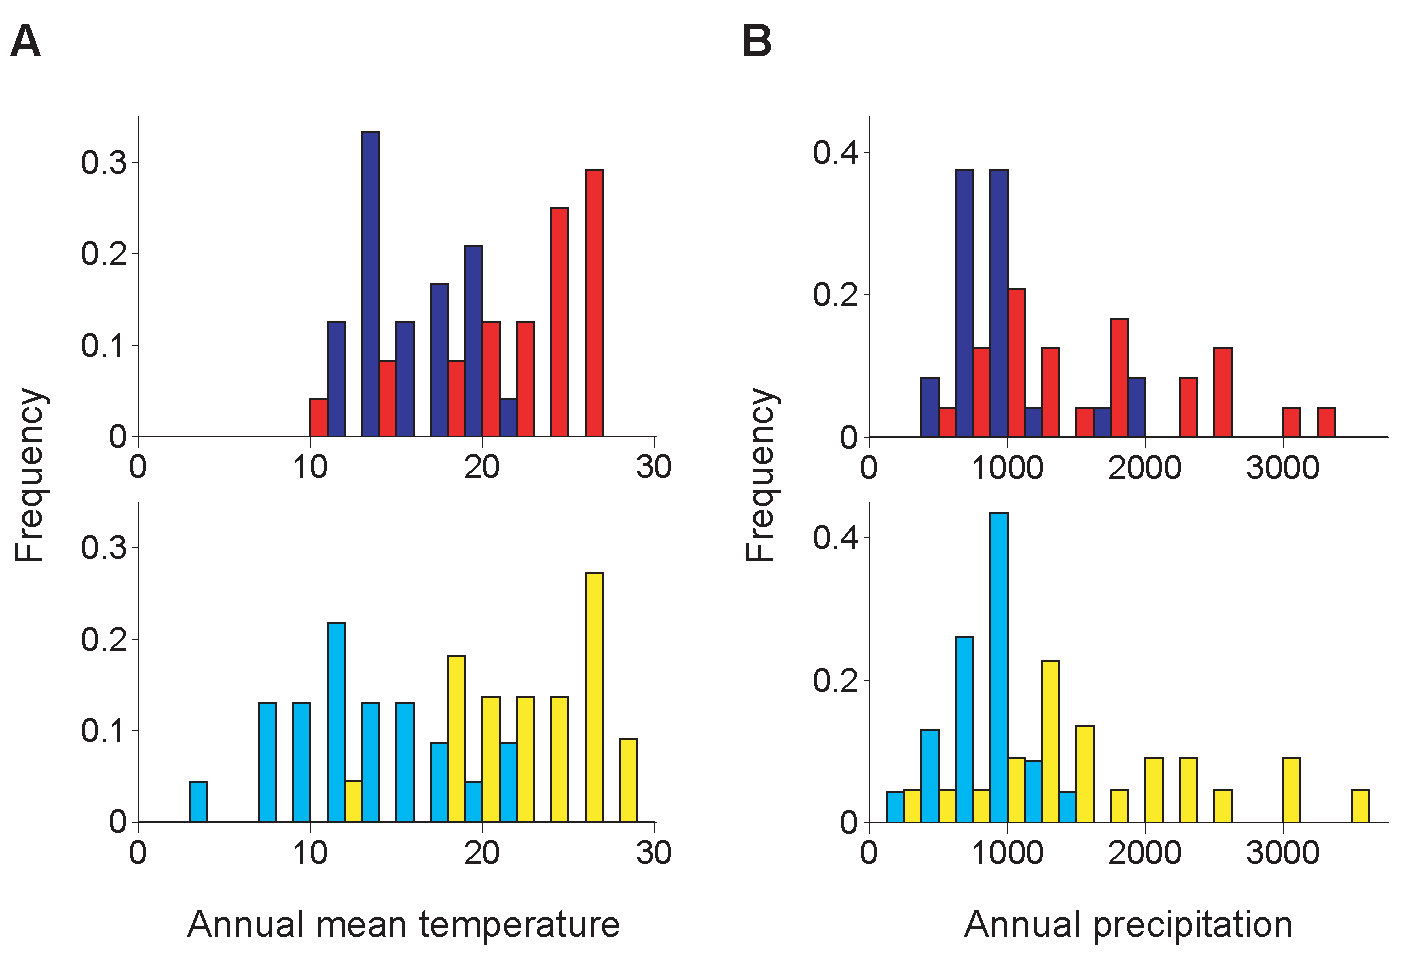
\includegraphics[width=0.5\columnwidth]{fig/bioclm.pdf}
    \caption{Annual mean temperature and annual precipitation of the  locations of the maize samples used in this study.
    Red, blue, yellow and light blue bars represent Mesoamerican lowland, Mesoamerican highland, S. American lowland and S. American highland
    populations, respectively.  
    }
    \label{supp:colfreq}
  \end{center}
\end{figure}
%%%%%%%%%%%%%%%%%%%%%%%%%%%%%%%%%%%%%%%%%%%%%%%%%%%%%%%%%%%%

%%%%%%%%%%%%%%%%%%%%%%%%%%%%%%%%%%%%%%%%%%%%%%%%%%%%%%%%%%%%
\begin{figure}[h]
  \begin{center}
    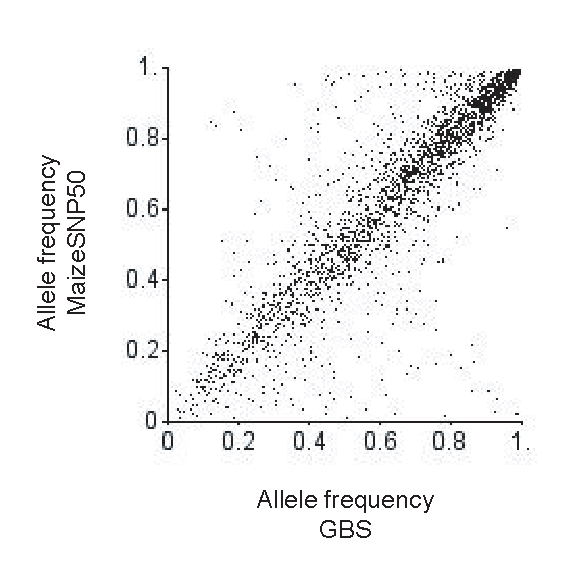
\includegraphics[width=0.4\columnwidth]{fig/Col.pdf}
    \caption{Correlation of allele frequencies between GBS and MaizeSNP50  data.  We used overlapping SNPs with $n\geq40$ for both data sets.  The correlation coefficient is 0.890 ($P<10^{-5}$ by permutation test with $10^5$ replications).}
    \label{supp:correl_freq}
  \end{center}
\end{figure}
%%%%%%%%%%%%%%%%%%%%%%%%%%%%%%%%%%%%%%%%%%%%%%%%%%%%%%%%%%%%

%%%%%%%%%%%%%%%%%%%%%%%%%%%%%%%%%%%%%%%%%%%%%%%%%%%%%%%%%%%%
\begin{figure}[h]
  \begin{center}
    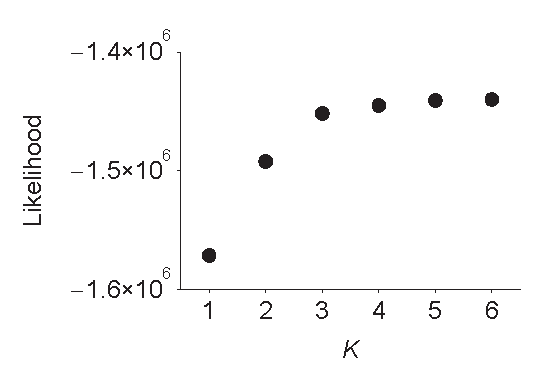
\includegraphics[width=0.4\columnwidth]{fig/kk.pdf}
    \caption{Likelihood of STRUCTURE analyses given the number of populations $K$.}
    \label{supp:struct}
  \end{center}
\end{figure}
%%%%%%%%%%%%%%%%%%%%%%%%%%%%%%%%%%%%%%%%%%%%%%%%%%%%%%%%%%%%

%%%%%%%%%%%%%%%%%%%%%%%%%%%%%%%%%%%%%%%%%% FIGURE
\begin{figure}[h]   
  \begin{center}
   \vspace{-0mm}
   %\includegraphics[width=0.23\textwidth]{figs/model}
   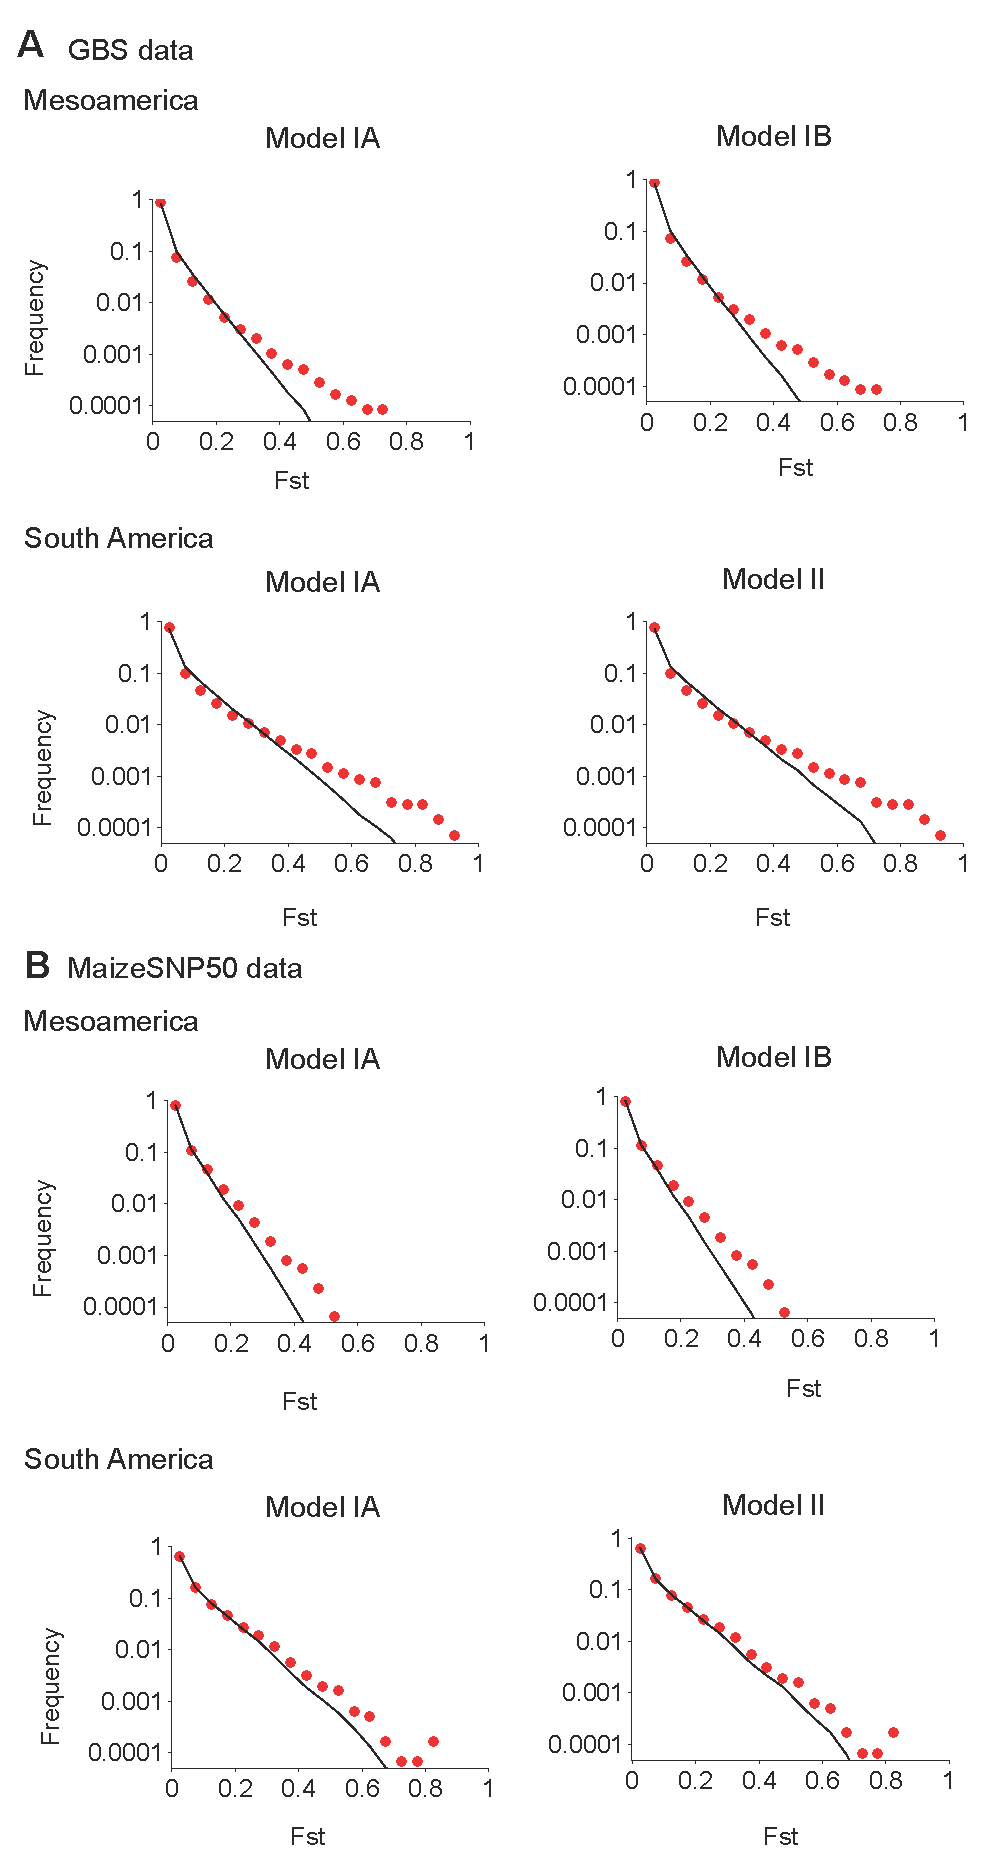
\includegraphics[width=0.45\textwidth]{fig/Fig5}
   \renewcommand{\baselinestretch}{0.9}
   \vspace{-3mm}
   \caption{Observed and expected distributions of $F_{ST}$ values in GBS (A) and MaizeSNP50 data (B).   The \emph{y}-axes represent the expected (solid lines) and observed (red dots) frequency of SNPs for a range of $F_{ST}$ values in bins of 0.05. 
   }
\vspace{-6mm}
    \label{FstDist}
  \end{center}
\end{figure}
%%%%%%%%%%%%%%%%%%%%%%%%%%%%%%%%%%%%%%%%%% FIGURE

%%%%%%%%%%%%%%%%%%%%%%%%%%%%%%%%%%%%%%%%%%%%%%%%%%%%%%%%%%%%
\begin{figure}[h]
  \begin{center}
    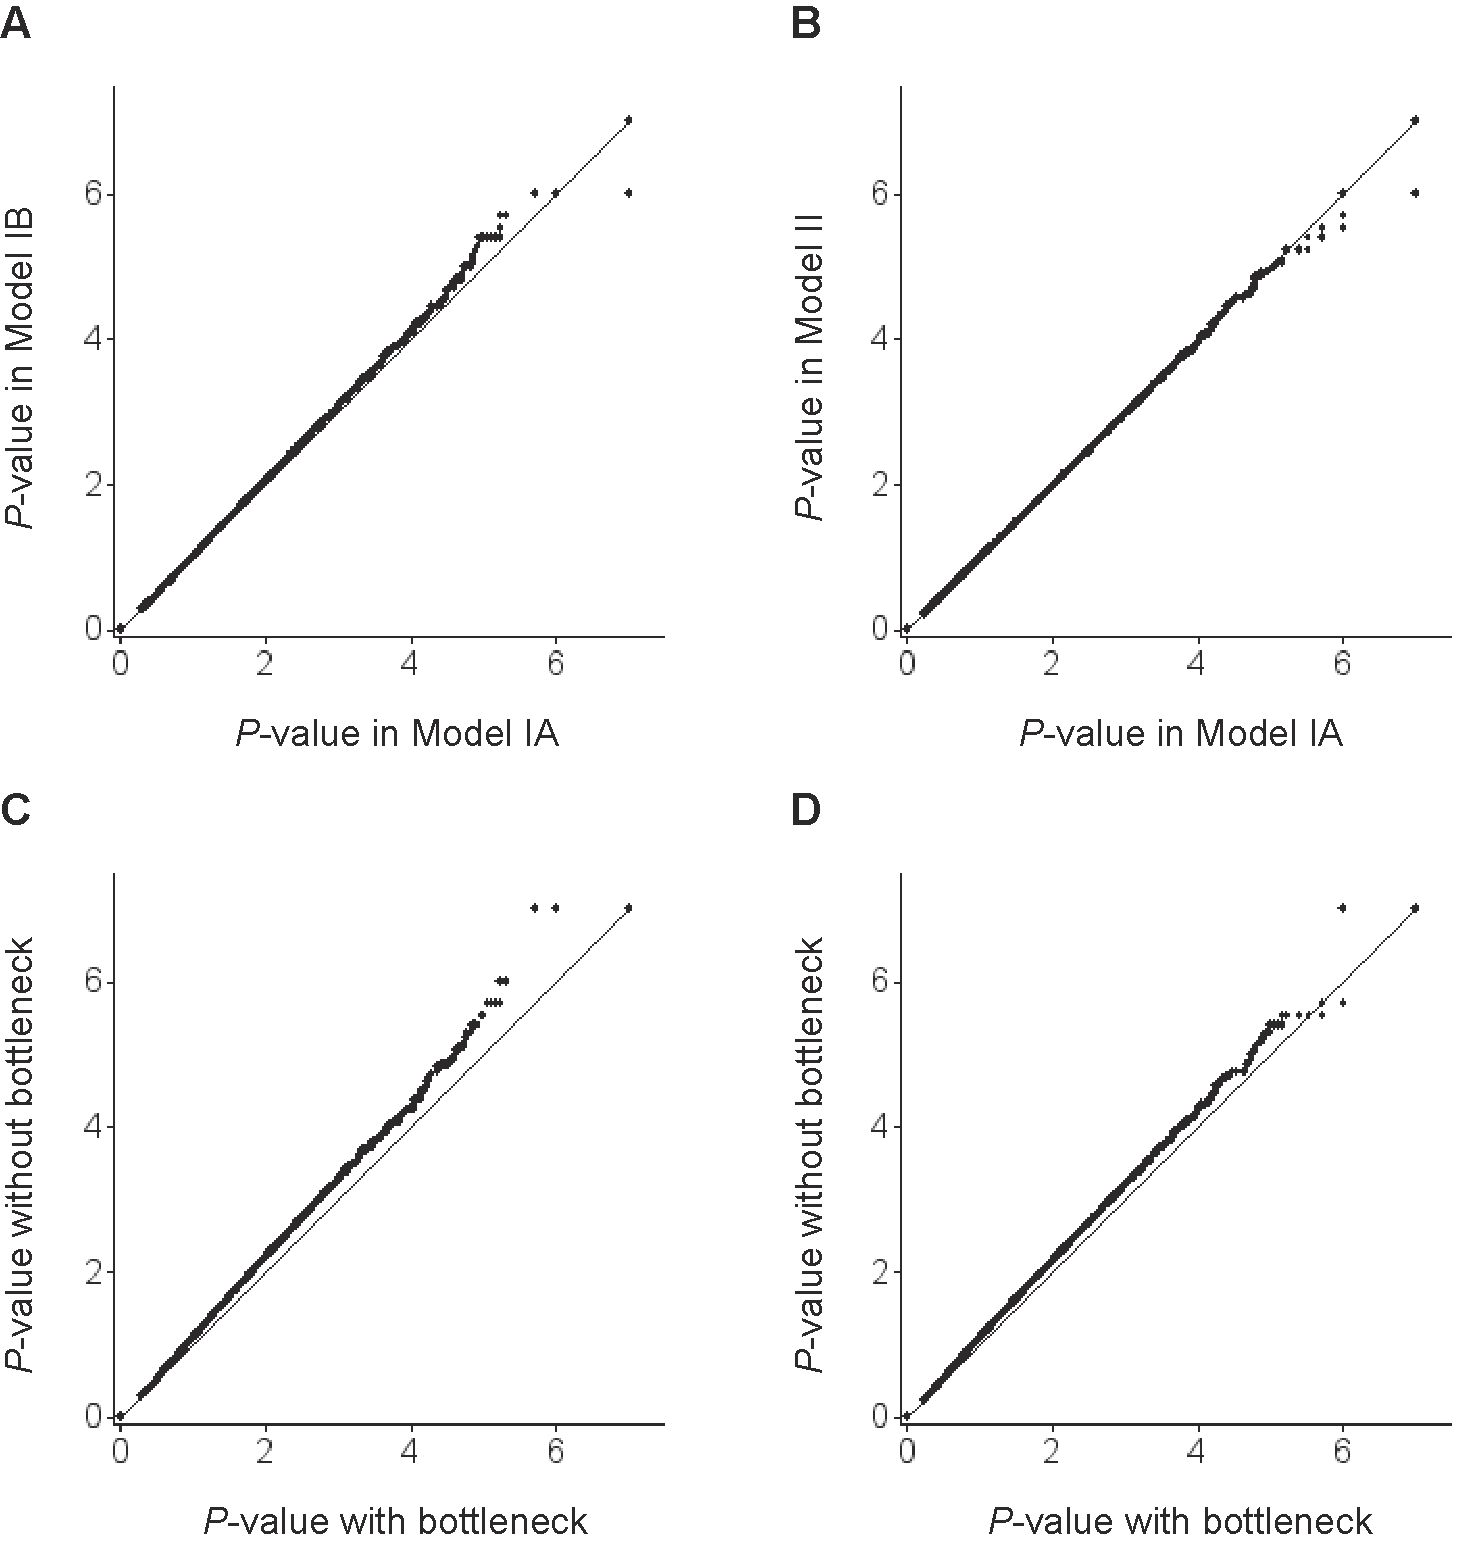
\includegraphics[width=0.6\columnwidth]{fig/bot2.pdf}
    \caption{Q-Q plot for $-$log$_{10}$-scaled \emph{P}-values of population differentiation between lowland and highland populations. (A) Model IA \emph{v.s.} Model IB in Mesoamerica, (B) Model IA \emph{v.s.} Model II in S. America.}
%    \caption{Q-Q plot for $-$log$_{10}$-scaled \emph{P}-values of population differentiation between lowland and highland populations. (A) Model IA \emph{v.s.} Model IB in Mesoamerica, (B) Model IA \emph{v.s.} Model II in S. America, (C) Model with \emph{v.s.} without bottleneck in Mesoamerica and (D) Model with \emph{v.s.} without bottleneck in S. America.}
    \label{fig:qq}
  \end{center}
\end{figure}
%%%%%%%%%%%%%%%%%%%%%%%%%%%%%%%%%%%%%%%%%%%%%%%%%%%%%%%%%%%%



%%%%%%%%%%%%%%%%%%%%%%%%%%%%%%%%%%%%%%%%%%%%%%%%%%%%%%%%%%%%
\begin{figure}[h]
  \begin{center}
    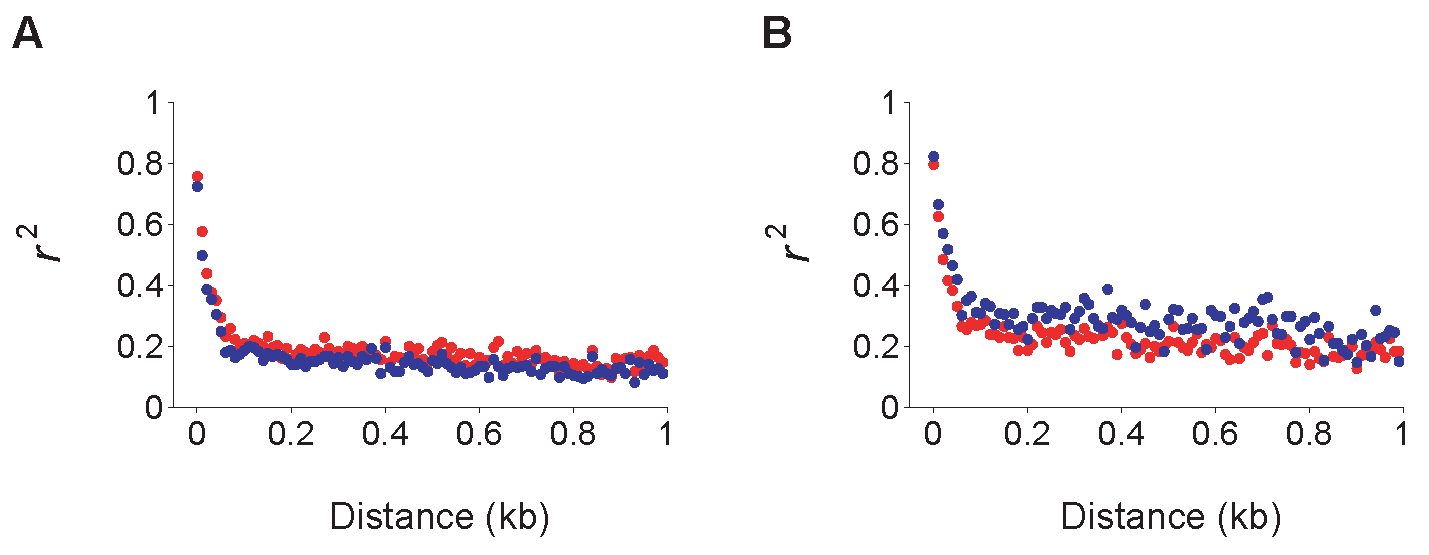
\includegraphics[width=0.7\columnwidth]{fig/LD.pdf}
    \caption{Pattern of decay of linkage equilibrium in Mesoamerica (A) and S. America (B).  Red and blue dots represent low- and highland populations, respectively.  $r^2$ values were for all pairs of SNPs and reported as averages within 10-bp distance bins. }
    \label{supp:LD}
  \end{center}
\end{figure}
%%%%%%%%%%%%%%%%%%%%%%%%%%%%%%%%%%%%%%%%%%%%%%%%%%%%%%%%%%%%

%\newpage
%\suppl
%\section*{File S1}
%
%\section*{Directionality of adaptation} \label{sec:supptextsho}
%\noindent {\Large \textit{Text~S1} }
%
%We classified the patterns of allelic differentiation among highland and lowland populations in Mesoamerica and S. America together with the information of \emph{parviglumis} in an \emph{ad hoc} manner; the allelic differentiation pattern is consistent with highland or lowland adaptation scenario.  
%In Figure~\ref{AllelePat}, we illustrate the frequency of putative ancestral and derived alleles in the five populations, drawn by red and blue, respectively.
%
%First, we focus on the SNPs with the signature of adaptation only in Mesoamerican populations (Figure~\ref{AllelePat}A).  
%\st{In other words, the $F_{ST}$ $P$-value is significant in Mesoamerica but not in S. America.
%The first and second rows show the typical patterns of highland adaptation in Mesoamerica with \emph{parviglumis} data available.
%We simply assume that the major allele in \emph{parviglumis} is ancestral. }
%Both rows show the consistent pattern to highland adaptation in Mesoamerica because the frequency of the putative derived allele in Mesoamerican highlands is highly differentiated from those in both \emph{parviglumis} and Mesoamerican lowlands.
%The patterns in S. America are different between the first and second rows.
%\st{Actually, in the second row, the frequency of the derived allele is increased also in S. American highland population. 
%However, we do not take the patterns in S. American populations into account because there is no adaptive signature in S. America (i.e., the $F_{ST} P$-value is not significant in S. America).}
%On the other hand, we should consider the allelic pattern in S. America in the case of the third row; we cannot utilize the information of \emph{parviglumis}.
%It is impossible to infer the ancestral allele, so we assume the pattern is consistent with highland adaptation if one allele is in higher frequency in Mesoamerican lowlands and S. American populations and the other is in higher frequency in Mesoamerican highlands.
%We classified the SNPs into lowland adaptation in the same way (from fourth to sixth rows in Figure~\ref{AllelePat}A).
%
%Next, we consider the SNPs with the signatures of adaptation in both Mesoamerica and S. America (Figure~\ref{AllelePat}B).
%The pattern in the first row is consistent with parallel highland adaptation, whereas the second row shows parallel lowland adaptation. 
%We cannot infer lowland or highland adaptation without the outgroup, so we ignore such SNPs.
%The pattern in the third row is the special case: the allele frequency is similar between Mesoamerican lowlands and S. American highlands and similar between Mesoamerican highlands and S. American lowlands.
%This pattern could be explained by that the SNP is linked to a red adaptive SNP and recombination breaks down the linkage between them.}

%\renewcommand{\thefigure}{\Roman{figure}}
%\setcounter{figure}{0}

%%%%%%%%%%%%%%%%%%%%%%%%%%%%%%%%%%%%%%%%%%%%%%%%%%%%%%%%%%%%
%\begin{figure}[b]
%  \begin{center}
%    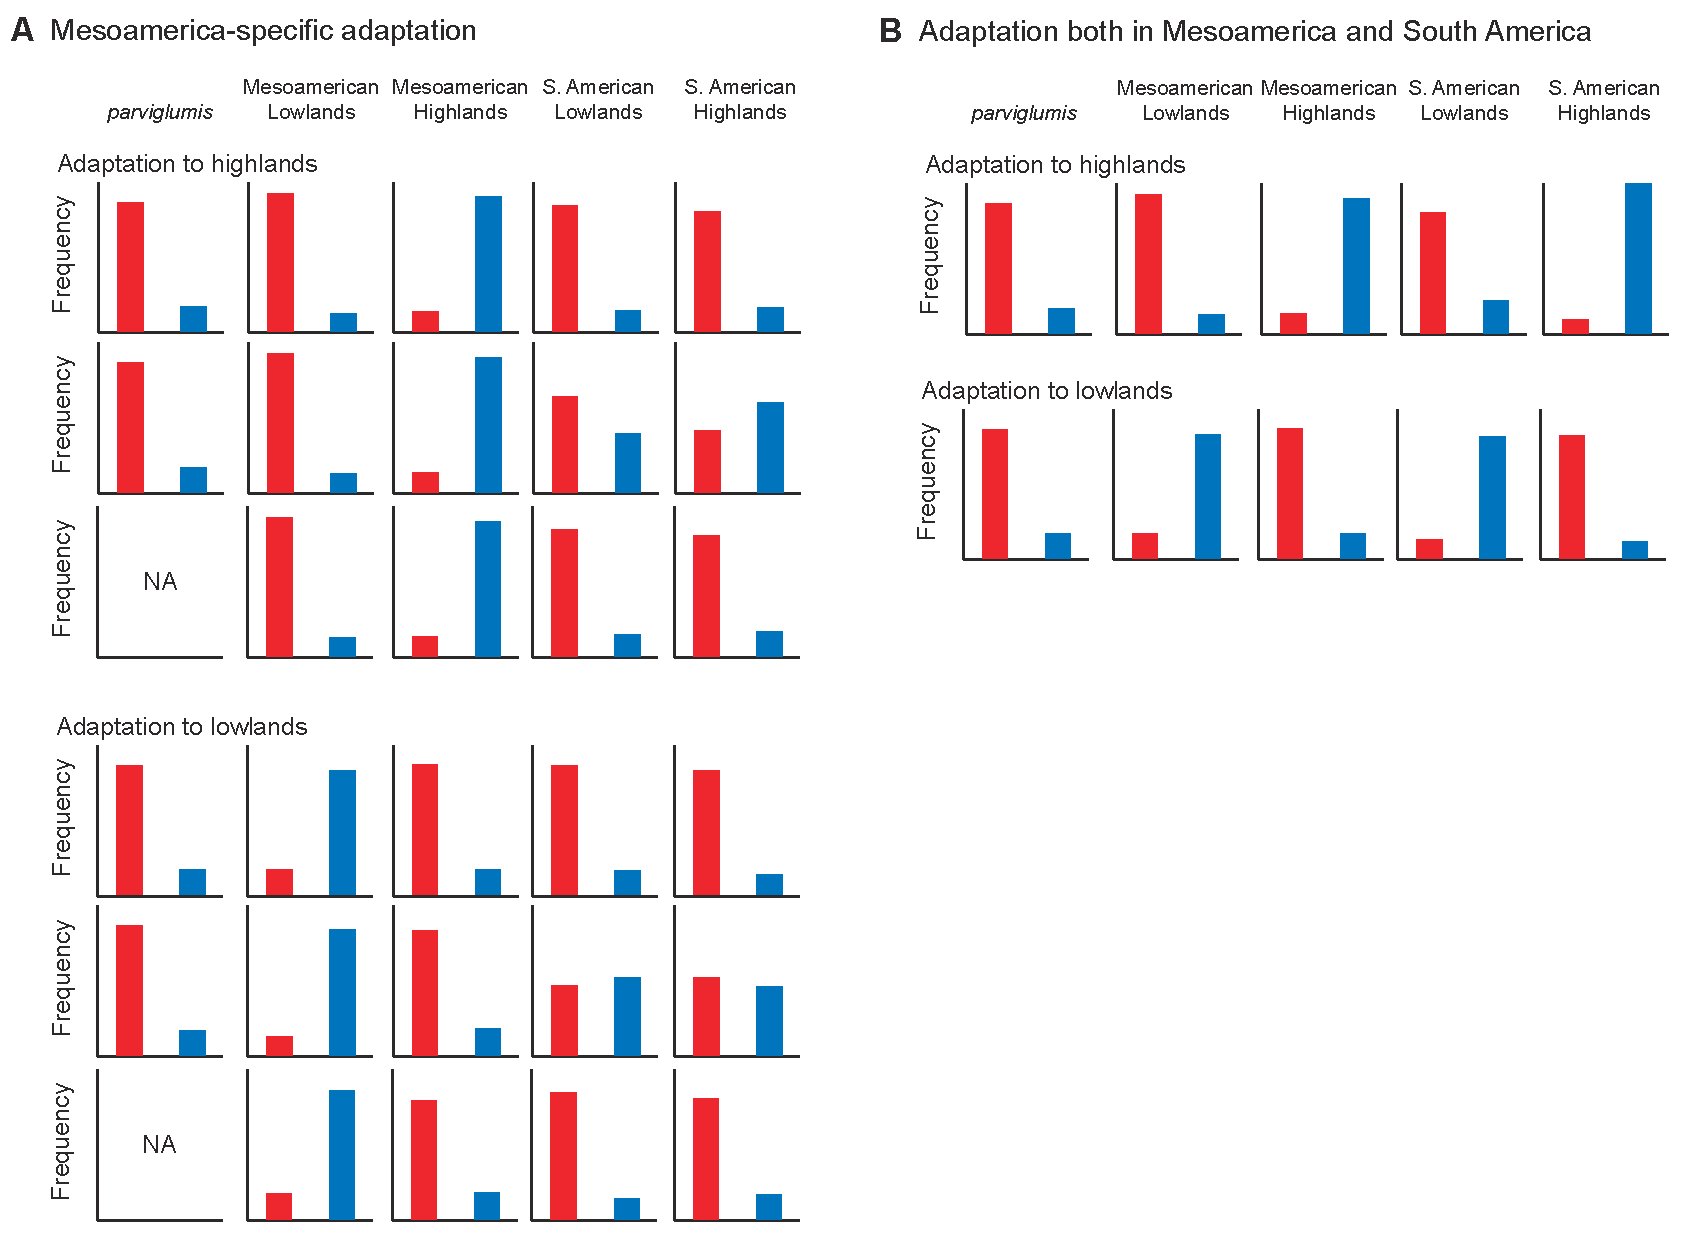
\includegraphics[width=0.9\columnwidth]{fig/AllelePat.pdf}
%    \caption{Illustration of allele frequency changes in maize and \emph{parviglumis}.  Red and blue bars represent the allele frequency of ancestral and derived, adaptive alleles, respectively.  The allele frequencies in the five populations are shown: \emph{parviglumis}, Mesoamerican lowlands and highlands, and S. America lowlands and highlands. NA in \emph{parviglumis} indicates that there is no SNP data in the site.  See the text for details. }
%    \label{AllelePat}
%  \end{center}
%\end{figure}
%%%%%%%%%%%%%%%%%%%%%%%%%%%%%%%%%%%%%%%%%%%%%%%%%%%%%%%%%%%%















